\documentclass[10pt,a4paper]{article}
\usepackage[utf8]{inputenc}
\usepackage{times}
\usepackage{courier}
\usepackage{graphicx}
\usepackage{hyperref}
\usepackage{courier}

\newcommand{\code}[1]{\texttt{#1}}

\title{Implementační dokumentace k \textbf{1}. úloze do IPP 2023/2024}
\author{Jméno a příjmení: \textbf{Jakub Všetečka} \\ Login: \textbf{xvsete00}}
\date{}

\begin{document}

\maketitle

\section{Design Philosophy}
The script is designed with an emphasis on modular architecture and object-oriented principles. The system comprises various classes like \code{XMLGenerator}, \code{Argument}, \code{Instruction}, \code{ArgumentParser}, and \code{InstructionParser}, each serving a distinct role, thereby promoting code reuse and ease of maintenance. The pipeline of the script is visualized in the figure~\ref{fig:pipeline}.

\begin{figure}[h]
\centering
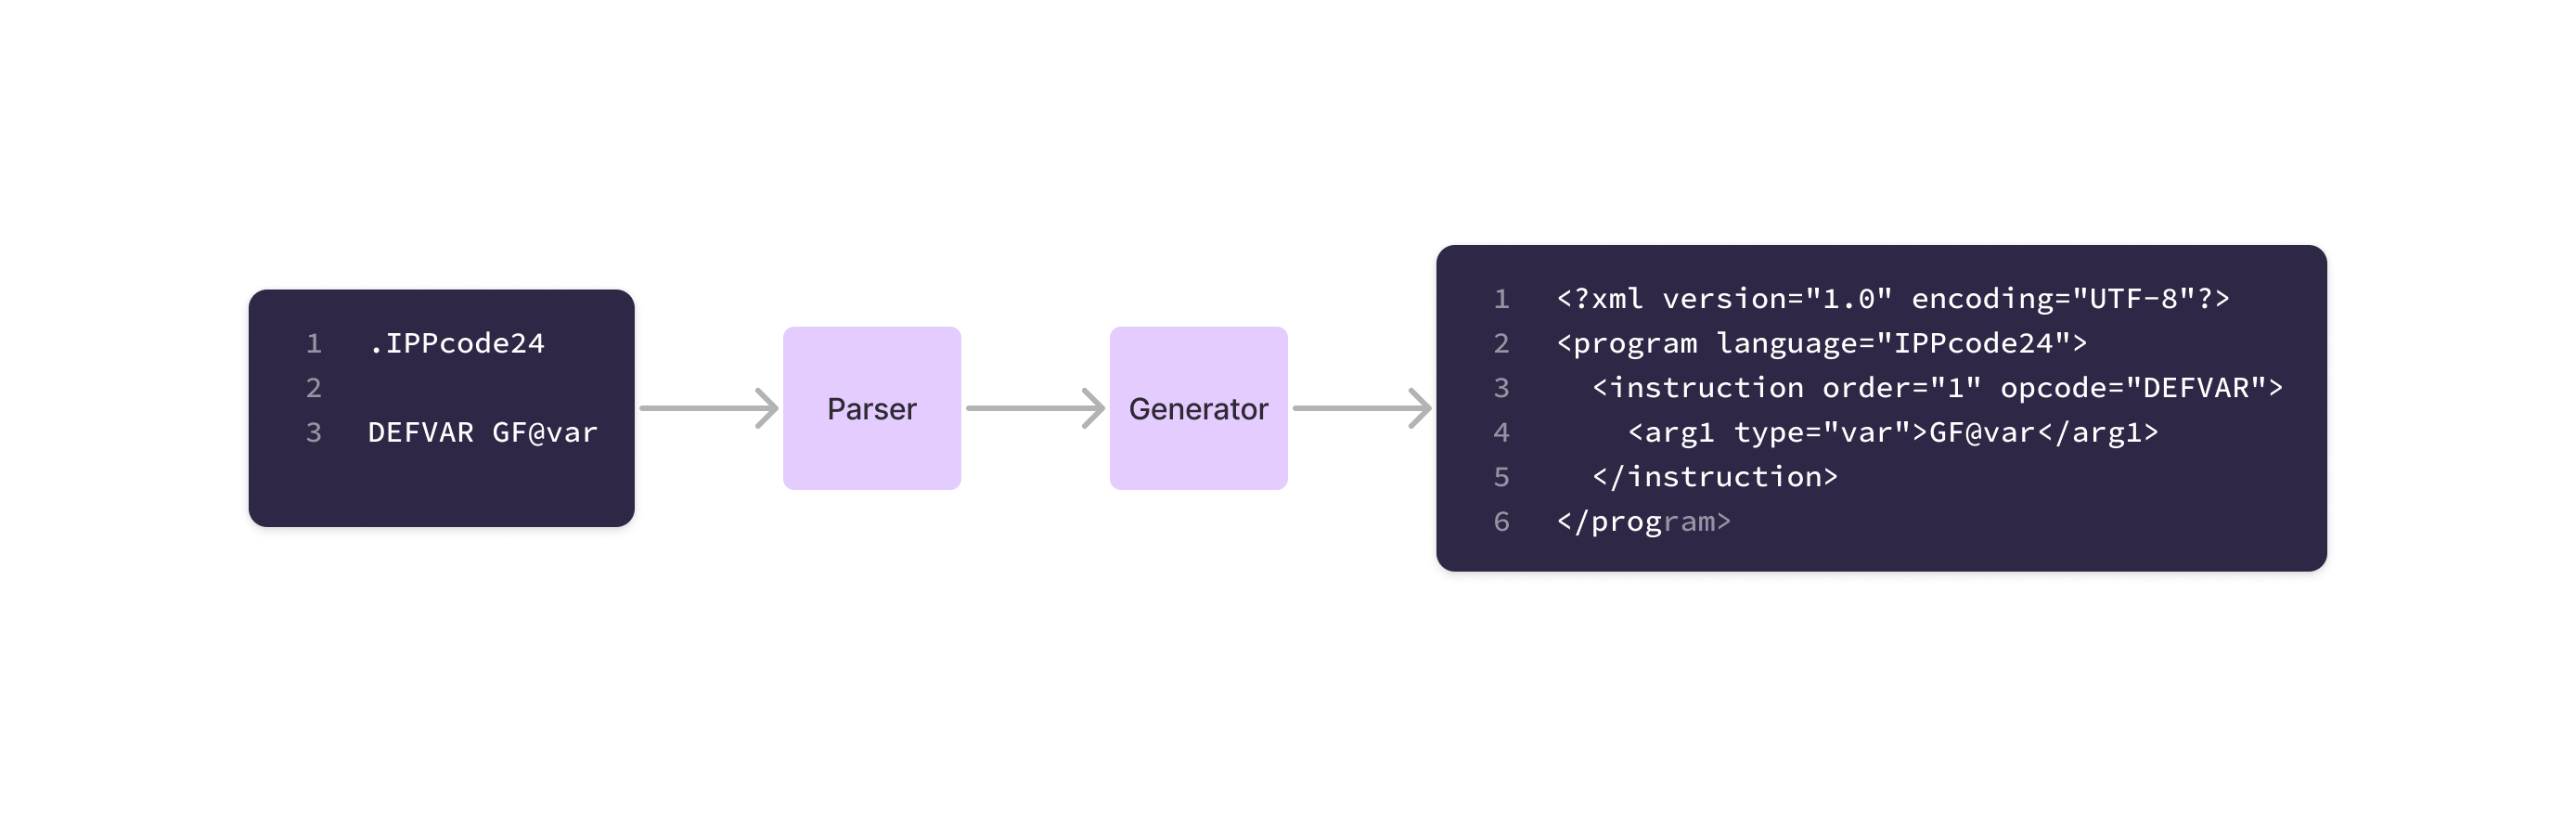
\includegraphics[width=\textwidth]{imgs/design.png}
\caption{Pipeline}
\label{fig:pipeline}
\end{figure}

\section{Internal Representation}
Each script component is represented as an object. \code{XMLGenerator} handles the XML structure, creating a skeleton for the output. Instructions and their arguments, encapsulated within their respective classes, act as building blocks for the script's functionality. The \code{ArgumentParser} and \code{InstructionParser} manage input parsing, transforming text into structured data. Enums ensure consistency in defining argument types and instruction formats, aiding in clear, manageable code. These objects are more closely detailed in the class
diagram~\ref{fig:classes}.

\begin{figure}[h]
    \centering
    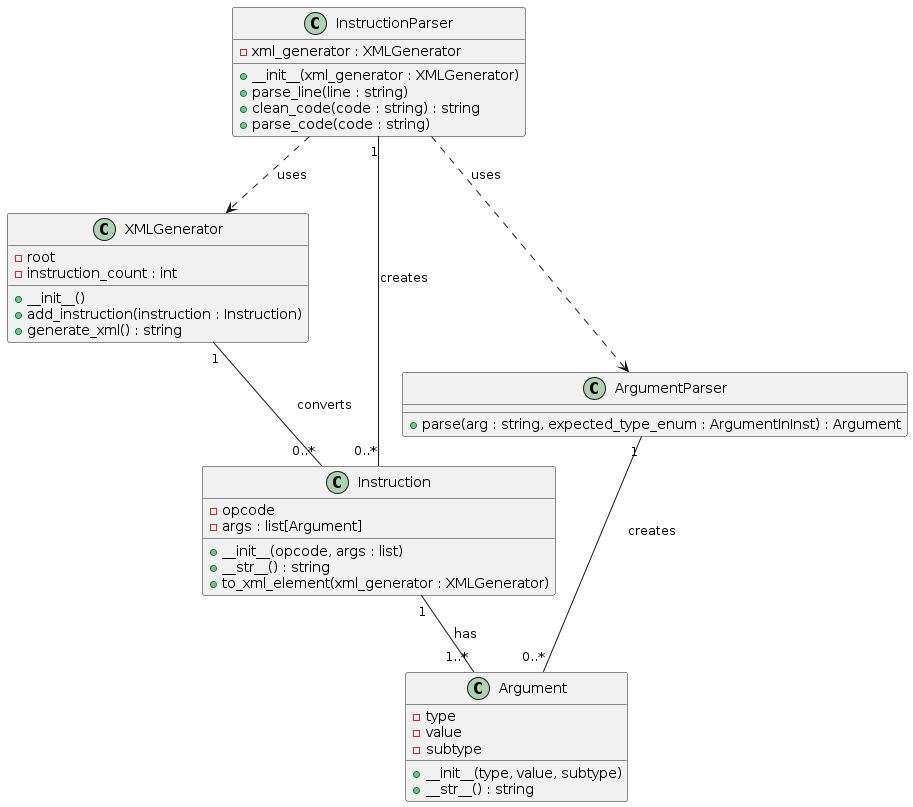
\includegraphics[width=\textwidth]{imgs/classes.png}
    \caption{Class Diagram}
    \label{fig:classes}
    \end{figure}


\section{Solution Procedure}
The approach involves parsing the input, building an internal representation, and outputting an XML document. The script begins by cleaning the input using \code{InstructionParser}, which employs regular expressions to remove extraneous elements like comments and unnecessary whitespace. It then leverages enums defined for argument types and instruction formats to facilitate regex-based parsing of instructions, identifying and validating each component of
instruction. After parsing, Instruction objects are created, which are subsequently used by \code{XMLGenerator} to construct the XML output.

\end{document}
